\documentclass[a4paper,11pt]{article}

%=========================
% Les styles
%=========================
\usepackage{style-esi/french}	% Francise LaTeX
\usepackage{style-esi/td}
\usepackage{style-esi/licence}	% Affiche une licence dans le document
\usepackage{style-esi/exercice}
\usepackage{style-esi/listing}
\usepackage{style-esi/tutoriel}
%\marginsectiontrue
\usepackage{booktabs}
\usepackage{pifont} 
%\usepackage{tabularx} 
%\usepackage{multicol}
%\usepackage{multirow}
\usepackage{longtable}
%\usepackage{array}

\definecolor{verylightgray}{rgb}{0.98,0.98,0.98}

\date{2018 -- 2019}
\siglecours{DEV1}
\libellecours{Laboratoires d'environnement}
\libelledocument{TD 03 -- L'éditeur de texte nano}
\sigleprof{}



\begin{document}

\entete
\titre
\ccbysa{esi-dev1-list@he2b.be}
\lastedit


	%===================
	%  Contenu
	%====================
	\begin{tcolorbox}[blanker,
	before skip=10mm,after skip=10mm,
	borderline west={1mm}{-4mm}{lightgray},
	title=Objectifs, coltitle=black, fonttitle=\sffamily\bfseries\large]
	Ce TD a pour objectif de vous familiariser avec l'éditeur \verb_nano_ \`a travers l'\'edition de vos premiers programmes simples.  
	\end{tcolorbox}
	
	\tableofcontents

	\newpage


%%%%%%%%%%%%%%%%%%%%%%%%%%%%%%%%%%%%%%%%%%%%%%%%%%%%%%%%%%%%%%%%%%%%%%%%%%%%%%%%%%%%%	   
\section{TD3 - L'éditeur de texte nano}
%%%%%%%%%%%%%%%%%%%%%%%%%%%%%%%%%%%%%%%%%%%%%%%%%%%%%%%%%%%%%%%%%%%%%%%%%%%%%%%%%%%%%
	 \begin{consigne}
	 	\begin{itemize}
			\item Ce TD est accompagn\'e d'exercices \`a faire \textbf{avant} de venir au laboratoire.
			\item Prenez bien note des r\'eponses aux exercices ainsi que de la fa\c con dont vous avez trouv\'e ces r\'eponses.
		\end{itemize}				
	\end{consigne}
	
%%%%%%%%%%%%%%%%%%%%%%%	
	\subsection{La ligne de commande}
%%%%%%%%%%%%%%%%%%%%%%%%
	
		\textbf{Dans votre r\'epertoire home, cr\'eez un r\'epertoire td3. Ce r\'epertoire contiendra tous les programmes Java que vous \'ecrirez aujourd'hui. 
		D\'esormais, vous prendrez cette habitude pour chaque td.}
            	
		\par
        
         	 Parfois, vous devez entrer une commande assez longue parce que les noms de fichiers sont longs et/ou nombreux.
          	Linux offre plusieurs facilit\'es pour simplifier l'entr\'ee de longues commandes.  
        
            	\par
        
			
		\begin{Tutoriel}{La compl\'etion de la commande} 
	          	Lorsque vous appuyez sur la touche \,\verb|TAB|\,, le shell tente de compl\'eter le d\'ebut de commande que vous avez d\'ej\`a tap\'e. 
			Si plusieurs possibilit\'es existent, elles sont affich\'ees si vous appuyez 2x sur  \,\verb|TAB|\,.  
        
            	\par
        		          Supposons que vous ne vous rappeliez plus tr\`es bien de la commande qui permet de modifier le mot de passe.
		          Vous vous rappelez juste qu'elle commence par \,\verb|pas|\,.  
        
            		\par
        
			\begin{steps}
				\item Tapez \,\verb|pas|\, puis appuyez 2x sur la touche \,\verb|TAB|\,.
				\item Entrez un \,\verb|s|\, puis appuyez \`a nouveau sur \,\verb|TAB|\,.
          		\end{steps}
		
		\end{Tutoriel}		
			
		\begin{Exercice}{La compl\'etion des noms de fichiers} 
		          La touche de tabulation permet \'egalement de compl\'eter un nom de fichier. 
			\begin{enumerate}
				\item Dans votre dossier td3, copiez le fichier \par
					\verb@monfichieraunomtellementlongquilmeparaitpeuprobabledeletaper2xsanserreur@ 
					qui se trouve dans le dossier \verb@/eCours/java/td/td3@.
          			\item Affichez le contenu de ce fichier en \'evitant de retaper son nom.
			\end{enumerate}
		\end{Exercice}	
		
		\begin{Exercice}{Joker} 
			Le point 20 du guide visuel parle des jokers; c'est le moment de les utiliser :) 
			\par
			\begin{enumerate}
				\item Copiez dans votre r\'epertoire td3 cr\'e\'e ci-dessus tous les fichiers du r\'epertoire \verb@/eCours/java/td/td3@ dont l'extension est \verb@.java@ 
				(c'est possible sans passer par un \,\verb|cd /eCours/java/td/td3|\,)
          		
            			\item Copiez dans votre r\'epertoire td3 tous les fichiers du r\'epertoire  \verb@/eCours@\ \verb@/java/td/td3@ dont la deuxi\`eme lettre est un '\verb@x@'.
 
 		      		\item  Listez le contenu des r\'epertoires des \'etudiants (pour rappel, les r\'epertoires des \'etudiants sont ceux qui se trouvent dans \verb@/home@ et qui 						commencent par un '\verb@g@').
         			\item Listez le contenu des r\'epertoires des professeurs (pour rappel, les r\'epertoires des professeurs sont ceux qui se trouvent dans \verb@/home@ et qui 						sont compos\'es de 3 lettres).
          		\end{enumerate}
		\end{Exercice}
				
			
		\subparagraph{Revenir \`a une commande pr\'ec\'edente} 
		
			\textcolor{white}{.} \par
			Il arrive souvent qu'il faille entrer une commande qu'on a d\'ej\`a \'ecrite il y a peu (ou en tout cas fort proche de ce qu'on a d\'ej\`a \'ecrit). 
          		C'est l\`a que les fl\`eches viennent \`a notre secours.  
        
           		 \par
          
          		La fl\`eche vers le haut permet de revenir aux commandes pr\'ec\'edentes et de les modifier. \`A utiliser sans mod\'eration...  
        
            		\par
%%%%%%%%%%%%%%%%%%%%%%%%%%%%%%%		
	\subsection{Un programme correct}
%%%%%%%%%%%%%%%%%%%%%%%%%%%%%%%			
		\begin{Tutoriel}{Compiler / ex\'ecuter un programme} 
		          Commen\c cons par un programme correct et tentons de l'ex\'ecuter.  
        			\par
          		Le fichier \,\verb|/eCours/java/td/td3/Ex.java|\, contient un petit programme Java tout simple qui affiche un message de bienvenue. Nous allons l'ex\'ecuter.  
        
           		 \par
        
			\begin{steps}	
				\item Normalement, vous avez d\'ej\`a copi\'e ce fichier chez vous dans un dossier td3.
				\item Lisez-le et voyez si vous devinez ce qu'il fait.
				\item Compilez-le. \`A quoi correspond cette phase ? Quel(s) est (sont) le(s) fichier(s) cr\'e\'e(s) ? 
				\item Ex\'ecutez-le. 
			\end{steps}
			
		\end{Tutoriel}
%%%%%%%%%%%%%%%%%%%%%%%%%%%%%%%%%%		
	\subsection{Configurer l'\'editeur}
%%%%%%%%%%%%%%%%%%%%%%%%%%%%%%%%%%

		Un \'editeur de texte, m\^eme simple comme nano, peut apporter quelques facilit\'es dans l'\'ecriture de programmes.
		
            	\par
        
			
		\begin{Tutoriel}{Coloration sytaxique} 
       			La coloration syntaxique signifie utiliser des couleurs pour mettre en \'evidence certaines parties d'un code :
			mots cl\'es, constantes...
        
            		\par
        
			Pour utiliser cette facilit\'e, il faut configurer nano. Cette configuration se fait dans le fichier \verb@~/.nanorc@
            		\par
        
			\begin{steps}
				\item Tapez la commande : \,\verb|nano ~/.nanorc|\,
				\item Ajoutez-y la ligne : \,\verb|include "/usr/share/nano/java.nanorc"|\,
				\item Quittez l'\'editeur.
				\item Ouvrez le fichier \,\verb|Ex.java|\,. Il devrait \^etre color\'e.
			\end{steps}
		\end{Tutoriel}
				
			
		\begin{Tutoriel}{Num\'erotation des lignes} 
			Nano peut \'egalement indiquer le num\'ero de la ligne sur laquelle se trouve le curseur, ce qui sera pratique pour corriger vos erreurs. Pour cela,
			il existe deux m\'ethodes.
		
            		\par
        
			\begin{steps}
				\item Lancez nano avec l'option \verb@-c@ : \,\verb|nano -c monFichier|\,.
				\item Dans l'\'editeur, appuyez sur \,\verb|CTRL-c|\,.
			\end{steps}
		\end{Tutoriel}		
			
		\subparagraph{Indentation} 
		
			\textcolor{white}{.} \par
				 
			Pour qu'un programme soit lisible, il doit \^etre \textit{indent\'e}. Ce qui serait pratique lorsqu'on code ce serait qu'un retour \`a la ligne positionne
			automatiquement le curseur de fa\c con \`a \^etre align\'e avec la ligne pr\'ec\'edente. Pour que nano fasse \c ca pour nous, il suffit d'ajouter 
			ceci \`a son fichier de configuration : \,\verb|set autoindent|\,.
		
            		\par
        
			
		\subparagraph{Autres configurations} 
		
			\textcolor{white}{.} \par
				 
			Si vous d\'esirez connaitre d'autres possibilit\'es de configuration de nano, vous pouvez lire le manuel : \,\verb|man nanorc|\,.
		
            		\par
        

			Pour une \textit{quick ref} en ligne, consultez (par exemple) : \\
			http://www.codexpedia.com/text-editor/nano-text-editor-command-cheatsheet/\\
			 (\url{www.codexpedia.com/text-editor/nano-text-editor-command-cheatsheet/})
            		\par
        
			
		\begin{Tutoriel}{Exp\'erience} 
				\begin{steps}
					\item Allez dans votre \textit{home} et tapez la commande : \,\verb|nano .nanorc|\,.
						\par
						Vous pouvez sortir de l'\'editeur.
			
					\item Tapez la commande : \,\verb|ls|\,. Vous ne voyez pas le fichier \verb@.nanorc@ alors qu'il est bien pr\'esent puisque vous
						pouvez l'\'editer !?
						\par
						Il s'agit en fait d'un fichier \verb@caché@.
				\end{steps}
		\end{Tutoriel}
				
			
		\begin{Exercice}{Les fichiers cach\'es} 
			En Linux, tous les fichiers qui commencent par un point sont consid\'er\'es comme \textit{cach\'es}.
			Par d\'efaut, il ne sont pas montr\'es \`a l'utilisateur. C'est surtout utilis\'e pour des fichiers de configuration.
			Pour tout de m\^eme visualiser un fichier cach\'e, il faut utiliser une option de la commande \verb@ls@.
		
           		 \par
			\begin{itemize}
				\item Consultez la page de manuel de la commande \verb@ls@ et trouvez l'option qui permet de voir
					les fichiers cach\'es.
			\end{itemize}
		\end{Exercice}
            		\par
 %%%%%%%%%%%%%%%%%%%%%%%%%%%%%%%%%%%%%%%%
        \subsection{Mon premier programme}  
  %%%%%%%%%%%%%%%%%%%%%%%%%%%%%%%%%%%%%%%%
  
          	Vous allez \`a pr\'esent \'ecrire votre premier programme de bout en bout. Pour ne pas d\'eroger \`a la tradition, ce sera le \guillemotleft  Hello-World! \guillemotright    
          	(La plupart des manuels de pr\'esentation d'un langage commencent par ce grand classique !).  
        
           	 \par
          
          	Vous devez maintenant \^etre capable de faire \c ca tout seul, sans qu'on vous donne la r\'eponse. Mais si vous avez un probl\`eme, vous pouvez toujours 
		appeler votre professeur :)   
        
           	 \par
        
		\clearpage	
		\begin{Tutoriel}{Hello world} 					
			\begin{steps}
				\item \'Ecrivez votre premier programme nomm\'e \verb|Hello.java| qui affiche le message  \guillemotleft  Hello, world ! \guillemotright .
				\item Compilez-le et ex\'ecutez-le.
			\end{steps}
		\end{Tutoriel}		  
          	%Vous ne vous souvenez plus comment afficher  \guillemotleft  Hello World \guillemotright  \`a l'\'ecran ?  
        
          %  \par
        % {\footnotesize\emph{(le code \`a \'ecrire est disponible dans la version en ligne)}\par} 
			
%		\subparagraph{Au hasard} 
%		
%					\textcolor{white}{.} \par
%				
%            \par
%        
%					\begin{enumerate}
%				
%			\item \'Ecrivez le programme qui affiche un nombre r\'eel au hasard entre 0 inclus et 1 exclu. Compilez-le et ex\'ecutez-le.
%			\item Modifiez-le afin qu'il affiche un nombre r\'eel au hasard entre 0 inclus et 6 exclu. Compilez-le et ex\'ecutez-le.
%			\item Modifiez-le une nouvelle fois afin qu'il affiche un nombre r\'eel au hasard entre 1 inclus et 6 exclu.
%					\end{enumerate}

%%%%%%%%%%%%%%%%%%%%%%%%%%%%%%%%%%%%%%%%%%%%%
	\subsection{D\'etecter et corriger les erreurs}  
%%%%%%%%%%%%%%%%%%%%%%%%%%%%%%%%%%%%%%%%%%%%%
          	Jusque l\`a, vous avez pu travailler avec un programme correct. Voyons maintenant comment proc\'eder lorsque des erreurs apparaissent 
		(et \c ca ne manquera pas d'arriver !)   
        
            	\par
        
			
		\subparagraph{Comprendre une erreur de compilation} 
		
			\textcolor{white}{.} \par
          		Un r\^ole important de la compilation est de rep\'erer les erreurs lexicales et/ou syntaxiques que rec\`ele un fichier source 
         		 et de les d\'ecrire le plus clairement possible afin que le programmeur puisse y rem\'edier. 
         		 Il est important d'apprendre \`a comprendre ces messages d'erreur.   
        
            		\par
		
        			\begin{figure}[hbt]
				\begin{center}
					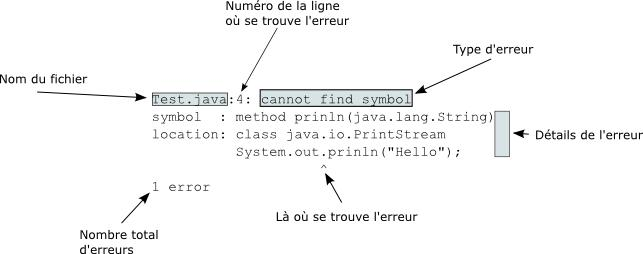
\includegraphics[width=0.8\linewidth,height=0.8\textheight,keepaspectratio=true]{image/ErreurCompil.jpg}
				\end{center}
                
                   		 \caption[Erreur de compilation]{Erreur de compilation}
               		 \end{figure}
                    
			
			\subparagraph{Comprendre une erreur d'ex\'ecution} 
		
				\textcolor{white}{.} \par
			          Lorsqu'on ex\'ecute une classe, la machine virtuelle va chercher un fichier ".class" correspondant puis l'ex\'ecuter. Il y a donc 2 types d'erreurs bien distincts :  
        
           			 \par
        
				\begin{itemize}
					\item soit il ne peut pas trouver le fichier ".class" demand\'e;
					\item soit il peut trouver une erreur lors de l'ex\'ecution de cette classe (division par z\'ero par exemple).
            					\par
						\begin{figure}[hbt]
				    			\begin{center}
								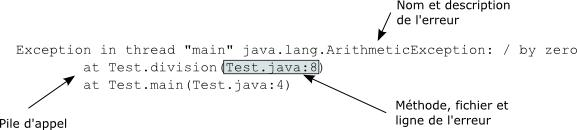
\includegraphics[width=0.8\linewidth,height=0.8\textheight,keepaspectratio=true]{image/ErreurExec.jpg}
							\end{center}
                
                   				 \caption[Erreur \`a l'ex\'ecution]{Erreur \`a l'ex\'ecution}
                					\end{figure}
                    
				\end{itemize}
				  
          			Le message d'erreur sera diff\'erent; apprenez \`a les reconnaitre.   
        
           			 \par
       				 \textbf{Note} : la qualit\'e d'un programmeur se voit surtout \`a sa capacit\'e \`a r\'eagir face aux erreurs. 
          			Prenez note des situations que vous allez rencontrer et des solutions afin de r\'eagir efficacement lorsque vous les rencontrerez \`a nouveau.  
        
           			 \par
        
			
			\begin{Exercice}{D\'etection des erreurs} 
			        Vous avez copi\'e dans votre r\'epertoire \verb@td3@ tous les fichiers \verb@.java@ se trouvant dans \verb@/eCours/java/td/td3@.  
        
            			\par
          
          			Hormis \verb@Ex.java@ utilis\'e pr\'ec\'edemment, tous ces fichiers sont erron\'es.  Les erreurs sont tant\^ot \`a la compilation, tant\^ot \`a l'ex\'ecution. Nous 					vous demandons de d\'etecter et de corriger les erreurs des programmes \textit{Ex1} \`a \textit{Ex12} et de noter le type d'erreur ainsi que le message 						engendr\'e.  
        
            			\par
        
				\par
               			 \begin{longtable}{|p{15.87mm}|p{15.876mm}|p{79.38mm}|}
                				\hline
					\endhead
        					\endfoot
        					 \bfseries Exercice \mdseries & \bfseries Erreur \mdseries & \bfseries Message affich\'e  \mdseries \\ \hline		
		 			\bfseries Ex1  \mdseries & & \\ \hline		
		 			\bfseries Ex2  \mdseries & & \\ \hline		
					 \bfseries Ex3 \mdseries & & \\ \hline		
		 			\bfseries Ex4 \mdseries & & \\ \hline		
		 			\bfseries Ex5  \mdseries & & \\ \hline		
					 \bfseries Ex6 \mdseries & & \\ \hline		
					 \bfseries Ex7 \mdseries & & \\ \hline		
		 			\bfseries Ex8 \mdseries & & \\ \hline		
					 \bfseries Ex9  \mdseries & & \\ \hline		
					 \bfseries Ex10 \mdseries & & \\ \hline		
				\end{longtable}
			\end{Exercice}
%		\subsection{Encore des programmes}
%          Voici quelques exercices qui vous permettrons aussi de d\'ecouvrir la classe Math.
%          https://docs.oracle.com/javase/8/docs/api/java/lang/Math.html (\url{https://docs.oracle.com/javase/8/docs/api/java/lang/Math.html})
%            \par
%        
%          Soyez attentifs \`a bien v\'erifier votre programme ;
%          ce n'est pas parce qu'il affiche quelque chose 
%          qu'il est correct !
%        
%            \par
%        
%			
%		\subparagraph{Afficher votre nom} 
%		
%					\textcolor{white}{.} \par
%				
%            \par
%          
%          \'Ecrire un programme qui affiche
%          votre nom. 
%        
%            \par
%        \clearpage  
%          \'Ecrire un programme qui calcule et affiche
%          la valeur des expressions suivantes:
%          
%					\begin{enumerate}
%				
%			\item 3421 + 756
%			\item 34 * 78
%			\item 1 + 6,9
%			\item 
%              7 exposant 2.  
%              Il n'existe pas d'op\'erateur pour l'exposant, comment vous en sortir autrement ?
%            
%			\item ((3+2)*(7*8))/(4*2)
%					\end{enumerate}
%				
%            \par
%        
%			
%		\subparagraph{2 exposant 10} 
%		
%					\textcolor{white}{.} \par
%				
%            \par
%          
%          \'Ecrire un programme qui calcule et affiche
%          la valeur de 2 exposant 10.
%          Il n'existe pas d'op\'erateur pour cela, vous devrez faire appel 
%          \`a la classe Math.
%        
%            \par
%        
%          Pour vous aider : exposant se dit aussi puissance, comment dit-on puissance en anglais ?
%        
%            \par
%        
%			
%		\subparagraph{Racine carr\'ee de 3} 
%		
%					\textcolor{white}{.} \par
%				
%            \par
%          
%          \'Ecrire un programme qui calcule et affiche
%          la racine carr\'ee de 3.
%          Il n'existe pas d'op\'erateur pour cela, vous devrez faire appel 
%          \`a la classe Math.
%        
%            \par

%%%%%%%%%%%%%%%%%%%%%%%%%%%%%%%%%%%%%%%%
        \subsection{Transfert de fichiers}  
 %%%%%%%%%%%%%%%%%%%%%%%%%%%%%%%%%%%%%%%%%
         	Vous n'avez peut-\^etre pas fini. Pour pouvoir continuer \`a la maison sans tout recommencer, 
         	il serait bon de pouvoir r\'ecup\'erer ce que vous avez d\'ej\`a fait sur linux1. \par
				
         	Il existe plusieurs m\'ethodes d\'ecrites dans l'aide-m\'emoire (dans le r\'epertoire \textit{aide}). \par
				
          	En voici une.  \par
				
            	\par
        \begin{Tutoriel}{Transférer des fichiers}
		\begin{steps}
				
			\item Ouvrez l'explorateur de fichier Windows (par exemple en cliquant sur l'ic\^one "My Computer").
			\item Dans le champ d'adresse, tapez l'adresse \,\verb_ftp://linux1_.
			\item Une boite de dialogue vous demande votre login et mot de passe (sur \textit{linux1}).
			\item Vous voyez apparaitre un dossier "linux1" qui correspond \`a votre dossier sur \textit{linux1}. 
			\item Vous pouvez y prendre/d\'eposer des fichiers comme vous le feriez pour un dossier Windows. 
            			Vous pouvez par exemple les mettre sur une \textbf{cl\'e USB}.
          
		\end{steps}
	\end{Tutoriel}			
				
				
\end{document}
			